\documentclass[UTF8,a4paper,12pt]{ctexart}

\usepackage{amsmath,amssymb}
\usepackage{geometry}
\usepackage{array,tabularx}
\usepackage{enumitem}
\usepackage{fancyhdr}
\usepackage{tikz}
\usepackage{lastpage}
\usepackage{xurl}
\usepackage[colorlinks=true, linkcolor=black, urlcolor=black]{hyperref}

\geometry{
  left=2.2cm,
  right=2.2cm,
  top=1.8cm,
  bottom=1.8cm
}

\setlength{\parindent}{0pt}
\setlength{\parskip}{0.5em}

\pagestyle{fancy}
\fancyhf{}
\renewcommand{\headrulewidth}{0pt}
\cfoot{\zihao{-5}第~\thepage~页~~共~\pageref{LastPage}~页}

\newcommand{\blank}[1][3cm]{\underline{\hspace{#1}}}
\newcommand{\fillblank}[2]{\underline{\makebox[#1][c]{#2}}}
\newcolumntype{C}[1]{>{\centering\arraybackslash}m{#1}}
\newcommand{\vennbox}{\draw[thin] (-1.45,-1.45) rectangle (2.95,1.45);}

\begin{document}

\thispagestyle{empty}

\begin{center}
    {\heiti\zihao{3} 说明}
\end{center}

\vspace{2em}

本份\underline{\textbf{信息论与编码原理}}期末试卷由 Fishplate 与一众志同道合的伙伴共同整理制作，内容主要来源于笔者参加 2026 年期末考试后的回忆。受记忆所限，部分题目的数据、措辞、选项排布和分值由笔者在\underline{\textbf{不改变考查内容与方向的前提下}}进行了合理补全。此外，由于原考试采用机考形式，本文档版式为自行设计，与真实考试存在差异。

\vspace{1em}

我校 2025—2026 学年信息论与编码原理期末考试采用机考形式。客观题从畅课中的 4 套包含20道客观题的题库中分别随机抽取 5 道，共 20 道，每题 2 分。本卷客观题共整理 33 道，来源包括本次考试回忆及历年留存题目，因此题目数量与标注总分并不完全对应。客观题仅供复习和查漏补缺使用，笔者不建议采用背题这种过拟合方式复习。

\vspace{1em}

本份试卷的答案部分均由ChatGPT-5.6 Sol生成，限于精力笔者无暇进行答案订正（2026鸣潮演唱会戒断反应中），因此答案仅供复习参考，其准确性请列位自行判断。如发现题目或答案存在错误，也欢迎大家进行补充、修改和校正。

\vspace{1em}

感谢竹木、vespergraine 等同学提供的考后回忆、题目细节与交叉印证，也感谢所有参与讨论和补充的同学。本文档能够最终整理成形，并留给后来的同学复习使用，离不开
大家的共同努力。



\begin{center}

{\heiti{功成不必在我，功成必定有我！}}

\end{center}


本试卷开源至 GitHub：\url{https://github.com/Pandamonic/CUC_2025-2026_InformationTheory_Final_Exam}，供同学们自由学习、复习和二次整理使用。如果发现有错误也欢迎大家在这里改正。

\vspace{1em}

\begin{center}

{\heiti{祝大家复习顺利，考试取得好成绩!}}

{\textbf{Per Aspera Ad Astra!}}

\vspace{1em}

{\heiti btw重要的事情说三遍：}

\vspace{1em}

{\heiti 本资料是免费的，如果你是花钱买到的，说明你被坑了！！}

{\heiti 本资料是免费的，如果你是花钱买到的，说明你被坑了！！}

{\heiti 本资料是免费的，如果你是花钱买到的，说明你被坑了！！}

\end{center}

\vfill

\begin{center}
Fishplate\\
2026 年 7 月 18 日于上海黄浦
\end{center}

\newpage


\begin{center}
    {\heiti\zihao{4} 中国传媒大学}\\[0.8em]
    {\heiti\zihao{3} \fillblank{1cm}{2025}—\fillblank{1cm}{2026} 学年第\fillblank{1.1cm}{2}学期期末考试试卷}
\end{center}

\vspace{1.8em}

\begin{tabular}{@{}p{0.51\textwidth}p{0.43\textwidth}@{}}
考试科目：\fillblank{3.8cm}{信息论与编码原理}
&
课程编号：\fillblank{3.8cm}{2111010031}
\\[1.1em]
考试班级：\fillblank{3.8cm}{24级信通学院各专业}
&
考试方式：\fillblank{3.8cm}{闭卷}
\\[-0.2em]
&
\end{tabular}

\begin{center}
\renewcommand{\arraystretch}{1.55}
\setlength{\tabcolsep}{4pt}
\begin{tabular}{|C{1.6cm}|*{5}{C{1.6cm}|}C{1.6cm}|}
\hline
题目 & 一 & 二 & 三 & 四 & 五  & 总分 \\
\hline
得分 &  &  &  &  &  &   \\
\hline
\end{tabular}
\end{center}

\vspace{2.8em}

\noindent
\begin{minipage}[t]{0.25\textwidth}
\renewcommand{\arraystretch}{1.5}
\begin{tabular}{|C{1.5cm}|C{2.3cm}|}
\hline
得分 & 评卷人 \\
\hline
\rule{0pt}{0.8cm}&  \\
\hline
\end{tabular}
\end{minipage}
\begin{minipage}[t]{0.72\textwidth}
\vspace{1.0cm}
\begin{center}
{\heiti 一、客观题（40分）}
\end{center}
\end{minipage}

\vspace{1.2em}


\begin{enumerate}[label=\arabic*., leftmargin=2em, itemsep=1.4em]

\item 汉明码是完备码，其伴随式个数与错误图样个数相同。

\begin{tabular}{@{}p{0.22\textwidth}p{0.22\textwidth}@{}}
A. 对 & B. 错
\end{tabular}


\item 对于时齐马尔可夫信源来说，极限熵不一定存在，还必须满足遍历性条件。

\begin{tabular}{@{}p{0.22\textwidth}p{0.22\textwidth}@{}}
A. 正确 & B. 错误
\end{tabular}


\item 已知维拉图中 $H(X)$ 表示为：
\begin{center}
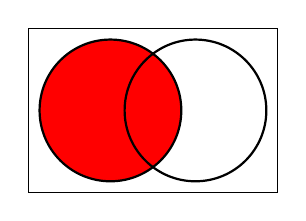
\begin{tikzpicture}[scale=0.72]
    \fill[red] (0,0) circle (1.25cm);
    \draw[thick] (0,0) circle (1.25cm);
    \draw[thick] (1.5,0) circle (1.25cm);
    \vennbox
\end{tikzpicture}
\end{center}

$H(Y)$ 表示为：

\begin{center}
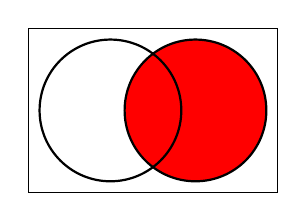
\begin{tikzpicture}[scale=0.72]
    \fill[red] (1.5,0) circle (1.25cm);
    \draw[thick] (0,0) circle (1.25cm);
    \draw[thick] (1.5,0) circle (1.25cm);
    \vennbox
\end{tikzpicture}
\end{center}

则 $H(Y|X)$ 表示为：

\begin{center}
\renewcommand{\arraystretch}{1.6}
\begin{tabular}{p{0.45\textwidth} p{0.45\textwidth}}

A.\ 
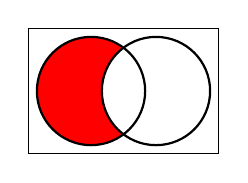
\begin{tikzpicture}[baseline=-0.5ex, scale=0.55]
    \fill[red] (0,0) circle (1.25cm);
    \fill[white] (1.5,0) circle (1.25cm);
    \draw[thick] (0,0) circle (1.25cm);
    \draw[thick] (1.5,0) circle (1.25cm);
    \vennbox
\end{tikzpicture}
&
B.\ 
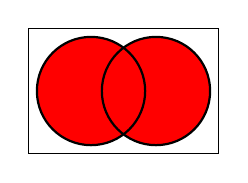
\begin{tikzpicture}[baseline=-0.5ex, scale=0.55]
    \begin{scope}
        \clip (0,0) circle (1.25cm);
        \fill[red] (-1.5,-1.5) rectangle (3,1.5);
    \end{scope}
    \begin{scope}
        \clip (1.5,0) circle (1.25cm);
        \fill[red] (-1.5,-1.5) rectangle (3,1.5);
    \end{scope}
    \draw[thick] (0,0) circle (1.25cm);
    \draw[thick] (1.5,0) circle (1.25cm);
    \vennbox
\end{tikzpicture}
\\

\vspace{1em}

C.\ 
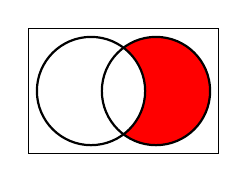
\begin{tikzpicture}[baseline=-0.5ex, scale=0.55]
    \fill[red] (1.5,0) circle (1.25cm);
    \fill[white] (0,0) circle (1.25cm);
    \draw[thick] (0,0) circle (1.25cm);
    \draw[thick] (1.5,0) circle (1.25cm);
    \vennbox
\end{tikzpicture}
&

\vspace{1em}

D.\ 
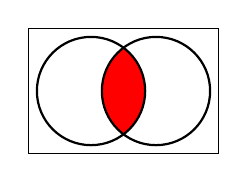
\begin{tikzpicture}[baseline=-0.5ex, scale=0.55]
    \begin{scope}
        \clip (0,0) circle (1.25cm);
        \fill[red] (1.5,0) circle (1.25cm);
    \end{scope}
    \draw[thick] (0,0) circle (1.25cm);
    \draw[thick] (1.5,0) circle (1.25cm);
    \vennbox
\end{tikzpicture}

\end{tabular}
\end{center}


\item 离散信道相关的所有概率（边缘概率、条件概率和联合概率）都可由下面选项中的哪两种概率表示？

\begin{enumerate}[label=\Alph*. , leftmargin=2em, itemsep=0.4em]
\item 信道输入概率 $p(x_i)$ 和信道转移概率 $p(y_j|x_i)$
\item 信道输入概率 $p(x_i)$ 和后验概率 $p(x_i|y_j)$
\item 信道输入概率 $p(x_i)$ 和输出概率 $p(y_j)$
\item 信道转移概率 $p(y_j|x_i)$ 和后验概率 $p(x_i|y_j)$
\end{enumerate}


\item 已知信道的输入是随机变量 $X$，输出随机变量是 $Y$，则信道的信息传输率 $R$ 等于：

\begin{tabular}{@{}p{0.22\textwidth}p{0.22\textwidth}p{0.22\textwidth}p{0.22\textwidth}@{}}
A. $H(Y)$
&
B. $I(X;Y)$
&
C. $H(Y)-H(X)$
&
D. $H(Y|X)-H(X)$
\end{tabular}


\item 从 $Y$ 获得的关于 $X$ 的平均信息量，用以下哪一个函数表示？

\begin{tabular}{@{}p{0.22\textwidth}p{0.22\textwidth}p{0.22\textwidth}p{0.22\textwidth}@{}}
A. $H(X|Y)$ & B. $I(X;Y)$ & C. $H(Y|X)$ & D. $H(XY)$
\end{tabular}


\item 下列有关数据处理定理或信息不增原理描述正确的是：（多选题）

\begin{enumerate}[label=\Alph*. , leftmargin=2em, itemsep=0.6em]

\item 任何无源处理过程（不涉及原始信源）一般总是丢失信息的，最多保持原来获得的信息不变，不可能比原来获得的信息还多。

\item 信息不增原理表明，只要对数据进行了处理了，不论怎么处理，都会丢失信息。

\item 在任何信息传输系统中，一旦在某一过程丢失一些信息，以后的系统不管如何处理，如不触及到丢失信息过程的输入端，就不能再恢复已丢失的信息。

\item 如果想从测量数据中获得更多关于 $X$ 的信息量，就必须进行有源处理。

\end{enumerate}

\item $I(X;X)=0$。

\begin{tabular}{@{}p{0.22\textwidth}p{0.22\textwidth}@{}}
A. 对 & B. 错
\end{tabular}


\item 以下关于霍夫曼编码的描述不正确的有：（多选题）

\begin{enumerate}[label=\Alph*. , leftmargin=2em, itemsep=0.4em]
\item 霍夫曼编码使信源符号近似等概率分布。
\item 霍夫曼编码的码组具有唯一性。
\item 霍夫曼码是即时码，也是最佳码。
\item 霍夫曼编码是从树根到树叶的编码过程。
\end{enumerate}


\item 定长码唯一可译的充要条件是满足非奇异性。

\begin{tabular}{@{}p{0.22\textwidth}p{0.22\textwidth}@{}}
A. 正确 & B. 错误
\end{tabular}


\item 离散级联信道如下图所示：

\begin{center}
\begin{tikzpicture}[>=stealth, thick]
    \node (x) at (0,0) {$X$};
    \node[draw, minimum width=1.5cm, minimum height=0.75cm] (c1) at (2,0) {信道 I};
    \node (y) at (3.4,0) {$Y$};
    \node[draw, minimum width=1.5cm, minimum height=0.75cm] (c2) at (4.8,0) {信道 II};
    \node (z) at (6.2,0) {$Z$};

    \draw[->] (x) -- (c1);
    \draw[->] (c1) -- (y);
    \draw[->] (y) -- (c2);
    \draw[->] (c2) -- (z);
\end{tikzpicture}
\end{center}

$X,Y,Z$ 构成马尔可夫链，则
\[
I(XY;Z)\ \blank[1.2cm]\ I(Y;Z),
\]
\[
I(X;Z)\ \blank[1.2cm]\ I(Y;Z),
\]
\[
P_{Z|X}\ \blank[1.2cm]\ P_{Y|X}P_{Z|Y}.
\]

依次应是：

\begin{enumerate}[label=\Alph*. , leftmargin=2em, itemsep=0.4em]
\item 大于等于，大于，小于
\item 等于，小于等于，等于
\item 小于，等于，大于
\item 小于等于，大于，等于
\end{enumerate}


\item 以下关于率失真函数的描述中不正确的是：

\begin{enumerate}[label=\Alph*. , leftmargin=2em, itemsep=0.4em]
\item 满足保真度准则的前提下，$R(D)$ 是信息率允许压缩到的下限。
\item $R(D)$ 是信源特有的参数。
\item 率失真函数是接收端以满足失真要求再现信源消息所必须获取的平均信息量的最小值。
\item 率失真函数的值域是 $[0,H(S)]$（其中 $H(S)$ 表示信源熵），是定义域上的严格递减函数。
\end{enumerate}


\item 条件熵 $H(Y|X)$ 计算错误的公式是：

\begin{enumerate}[label=\Alph*. , leftmargin=2em, itemsep=0.4em]
\item
$H(Y|X)
=
-\sum_i\sum_j p(y_j|x_i)\log p(y_j|x_i)
$

\item
$
H(Y|X)
=
-\sum_i\sum_j p(x_i y_j)\log p(y_j|x_i)
$

\item
$
H(Y|X)=H(XY)-H(X)
$

\item
$
H(Y|X)=H(Y)-H(X)+H(X|Y)
$
\end{enumerate}


\item 错误译码概率与信道的统计特性有关，也与译码规则有关。

\begin{tabular}{@{}p{0.22\textwidth}p{0.22\textwidth}@{}}
A. 正确 & B. 错误
\end{tabular}


\item 香农第一定理告诉我们平均码长的下界是香农熵（二进制编码时），并可以进一步推广到离散平稳信源编码。

\begin{tabular}{@{}p{0.22\textwidth}p{0.22\textwidth}@{}}
A. 对 & B. 错
\end{tabular}

\item 在求解马尔可夫信源极限熵时，可以不用验证马氏信源的遍历性，直接求解稳态概率。

\begin{tabular}{@{}p{0.22\textwidth}p{0.22\textwidth}@{}}
A. 对 & B. 错
\end{tabular}


\item 以下哪一项不是码符号序列译码二义性的存在条件？

\begin{enumerate}[label=\Alph*. , leftmargin=2em, itemsep=0.4em]
\item 存在前缀码。
\item 去除前缀码的剩余码可能和其他码字再次构成前缀码。
\item 码符号序列间尾部一定是一个码字。
\item 任意次扩展码都是非奇异码。
\end{enumerate}


\item 已知信道的输入是随机变量 $X$，输出是随机变量 $Y$，噪声熵用以下函数表示：

\begin{tabular}{@{}p{0.22\textwidth}p{0.22\textwidth}p{0.22\textwidth}p{0.22\textwidth}@{}}
A. $H(Y|X)$ & B. $H(X|Y)$ & C. $I(X;Y)$ & D. $H(Y)$
\end{tabular}


\item $(n,k)$ 循环码的非全零码字中连 $0$ 的个数最多只能有\blank[1.5cm]位。

\begin{tabular}{@{}p{0.22\textwidth}p{0.22\textwidth}p{0.22\textwidth}p{0.22\textwidth}@{}}
A. $n-k$ & B. $k$ & C. $n-1$ & D. $k-1$
\end{tabular}


\item 通信过程中降低传输错误概率的方法有：（多选题）

\begin{enumerate}[label=\Alph*. , leftmargin=2em, itemsep=0.4em]
\item 制定最佳的译码规则
\item 无失真信源编码
\item 改变信道的统计特性
\item 以上都可以
\end{enumerate}


\item Fano 不等式给出了错误概率的下限值，而选择好的译码规则可以使得错误概率达到最小值（不一定是下限值）。

\begin{tabular}{@{}p{0.22\textwidth}p{0.22\textwidth}@{}}
A. 对 & B. 错
\end{tabular}

\item 已知一信道转移概率图为：

\begin{center}
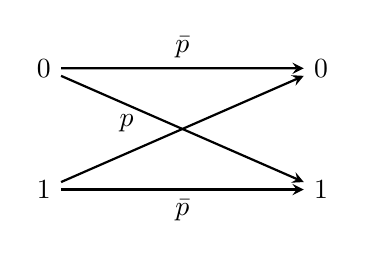
\begin{tikzpicture}[>=stealth, thick, scale=1.1]
    \node (x0) at (0,1.4) {$0$};
    \node (x1) at (0,0) {$1$};
    \node (y0) at (3.2,1.4) {$0$};
    \node (y1) at (3.2,0) {$1$};

    \draw[->] (x0) -- node[above] {$\bar p$} (y0);
    \draw[->] (x0) -- node[pos=0.27, below] {$p$} (y1);
    \draw[->] (x1) -- node[pos=0.27, above] {} (y0);
    \draw[->] (x1) -- node[below] {$\bar p$} (y1);
\end{tikzpicture}
\end{center}

请问该信道是：

\begin{enumerate}[label=\Alph*. , leftmargin=2em, itemsep=0.4em]
\item 二进制对称信道
\item 二进制删除信道
\item 有噪无损信道
\item 无噪有损信道
\end{enumerate}


\item 各维联合概率分布均与时间起点无关的信号称为平稳离散信源。

\begin{tabular}{@{}p{0.22\textwidth}p{0.22\textwidth}@{}}
A. 正确 & B. 错误
\end{tabular}


\item 关于自信息描述正确的选项是：（多选题）

\begin{enumerate}[label=\Alph*. , leftmargin=2em, itemsep=0.4em]
\item 收到消息获得的信息量等于不确定性减少的量。
\item 在理想信道中，等于收信者接收到该消息后所获取的信息量。
\item 事件发生前，描述该事件发生的不确定性的大小。
\item 事件发生后，表示该事件所含有的信息量。
\end{enumerate}


\item 对于已给 $(n,k)$ 线性分组码，伴随式数目与可纠正错误数量 $u$ 的关系为：
\[
2^{n-k}\ \blank[1.2cm]\ \sum_{i=0}^{u} C_n^i
\]

\begin{tabular}{@{}p{0.22\textwidth}p{0.22\textwidth}p{0.22\textwidth}p{0.22\textwidth}@{}}
A. $>$ & B. $\geq$ & C. $\leq$ & D. $<$
\end{tabular}

\newpage

\item 已知数字通信系统模型如下图所示：

\begin{center}
\begin{tikzpicture}[>=stealth, thick, xscale=1.0, yscale=1.0]
    \node[draw, minimum width=0.8cm, minimum height=1.2cm]
        (source) at (0,0) {\shortstack{信\\源}};

    \node[draw, minimum width=1.3cm, minimum height=0.75cm]
        (sc) at (1.8,0) {\shortstack{信源\\编码}};

    \node[draw, minimum width=1.3cm, minimum height=0.75cm]
        (cc) at (3.6,0) {\shortstack{信道\\编码}};

    \node[draw, minimum width=1.1cm, minimum height=0.75cm]
        (channel) at (5.3,0) {信道};

    \node[draw, minimum width=1.3cm, minimum height=0.75cm]
        (cd) at (7.0,0) {\shortstack{信道\\译码}};

    \node[draw, minimum width=1.3cm, minimum height=0.75cm]
        (sd) at (8.8,0) {\shortstack{信源\\译码}};

    \node[draw, minimum width=0.8cm, minimum height=1.2cm]
        (sink) at (10.4,0) {\shortstack{信\\宿}};

    \draw[->] (source) -- (sc);
    \draw[->] (sc) -- (cc);
    \draw[->] (cc) -- (channel);
    \draw[->] (channel) -- (cd);
    \draw[->] (cd) -- (sd);
    \draw[->] (sd) -- (sink);

    \node[below] (noise) at (5.3,-1.2) {噪声};
    \draw[->] (noise) -- (channel);
\end{tikzpicture}
\end{center}

其中，起到提高通信系统有效性作用的环节是？

\begin{tabular}{@{}p{0.22\textwidth}p{0.22\textwidth}p{0.22\textwidth}p{0.22\textwidth}@{}}
A. 信道 & B. 信源编码 & C. 信源 & D. 信道编码
\end{tabular}

\item 一离散信源有 $16$ 个符号，该信源的最大熵等于多少
$\mathrm{bit/}$符号？

\begin{tabular}{@{}p{0.22\textwidth}p{0.22\textwidth}p{0.22\textwidth}p{0.22\textwidth}@{}}
A. $2$ & B. $4$ & C. $6$ & D. $8$
\end{tabular}


\item 由定长编码定理可知，对于给定信源，当信源的序列长度 $N\to\infty$ 时，$\varepsilon$ 典型序列集合的概率趋于 $1$，非 $\varepsilon$ 典型序列集合的概率趋于 $0$。

\begin{tabular}{@{}p{0.22\textwidth}p{0.22\textwidth}@{}}
A. 对 & B. 错
\end{tabular}


\item 已知齐次马尔可夫信源的一步状态转移概率矩阵为
\[
P=
\begin{bmatrix}
0 & \dfrac{1}{2} & 0 & \dfrac{1}{2} \\[0.4em]
\dfrac{1}{2} & 0 & \dfrac{1}{2} & 0 \\[0.4em]
0 & \dfrac{1}{2} & 0 & \dfrac{1}{2} \\[0.4em]
\dfrac{1}{2} & 0 & \dfrac{1}{2} & 0
\end{bmatrix},
\]
则该马氏信源的稳态分布存在。

\begin{tabular}{@{}p{0.22\textwidth}p{0.22\textwidth}@{}}
A. 对 & B. 错
\end{tabular}

\item $N$ 维离散平稳信源的极限熵可以用（\hspace{1.2cm}）来计算：

\begin{tabular}{@{}p{0.22\textwidth}p{0.22\textwidth}p{0.22\textwidth}p{0.22\textwidth}@{}}
A. 单字符号熵 & B. $N$ 维联合熵 & C. $N-1$ 阶条件熵 & D. $N$ 阶条件熵
\end{tabular}


\item 以下关于信道编译码的描述中正确的有：（多选题）

\begin{enumerate}[label=\Alph*. , leftmargin=2em, itemsep=0.4em]
\item 信道编码是利用相关性来检测和纠正传输过程中产生的差错。
\item 信道译码是在接收到码符号序列后，按照与信道编码器相同的数学规律，检查并纠正错误，尽量还原符号序列。
\item 信道编码是按照一定的规则给信源编码后的码符号序列增加一些冗余信息，因而会降低通信的有效性。
\item 信道编码和信道译码是匹配的，因此没有信道编码，则无需信道译码。
\end{enumerate}


\item 互信息的计算公式，不正确的是：（多选题）

\begin{enumerate}[label=\Alph*. , leftmargin=2em, itemsep=0.4em]
\item $I(x_i;y_j)=I(y_j)-I(y_j|x_i)$
\item $I(x_i;y_j)=I(x_i)-I(y_j|x_i)$
\item $I(x_i;y_j)=I(y_j)-I(x_i|y_j)$
\item $I(x_i;y_j)=I(x_i y_j)-I(x_i)-I(y_j)$
\end{enumerate}


\item 由于干扰和噪声的存在，有噪无损信道无法实现端到端的无差错传输。

\begin{tabular}{@{}p{0.22\textwidth}p{0.22\textwidth}@{}}
A. 正确 & B. 错误
\end{tabular}


\end{enumerate}

\vspace{2.8em}

\noindent
\begin{minipage}[t]{0.25\textwidth}
\renewcommand{\arraystretch}{1.5}
\begin{tabular}{|C{1.5cm}|C{2.3cm}|}
\hline
得分 & 评卷人 \\
\hline
\rule{0pt}{0.8cm}&  \\
\hline
\end{tabular}
\end{minipage}
\begin{minipage}[t]{0.72\textwidth}
\vspace{1.0cm}
\begin{center}
{\heiti 二、（16分）}
\end{center}
\end{minipage}

\vspace{1.2em}

\noindent
设某二进制循环码的码长为 $7$，生成多项式为$g(x)=x^3+x+1$.

\begin{enumerate}[label=\arabic*., leftmargin=2.2em]
    \item 求该循环码的监督多项式 $h(x)$。

    \item 利用\textbf{余式法}构造\underline{系统码}的标准生成矩阵 $G$，并写出对应的校验矩阵 $H$。

    \item 求该码的最小汉明距离 $d_{\min}$，并说明其纠错能力和检错能力。

    \item 在\textbf{标准形式} （\underline{系统码}）校验矩阵下，设接收端分别收到
    \[
    Y_1=0001011
    \qquad\text{和}\qquad
    Y_2=0101110,
    \]
    分别对其进行纠检错。
\end{enumerate}

\newpage


\vspace{2.8em}

\noindent
\begin{minipage}[t]{0.25\textwidth}
\renewcommand{\arraystretch}{1.5}
\begin{tabular}{|C{1.5cm}|C{2.3cm}|}
\hline
得分 & 评卷人 \\
\hline
\rule{0pt}{0.8cm}&  \\
\hline
\end{tabular}
\end{minipage}
\begin{minipage}[t]{0.72\textwidth}
\vspace{1.0cm}
\begin{center}
{\heiti 三、（15分）}
\end{center}
\end{minipage}

\vspace{1.2em}

\noindent
某大型制造企业为了评估关键设备的健康度，需要对设备的运行状态进行连续监测。
根据设备运行机理，设备的运行状态主要分为四种：

\begin{center}
\renewcommand{\arraystretch}{1.4}
\begin{tabular}{@{}ll@{\qquad}ll@{}}
$S_1$： & 正常运行（Normal）
&
$S_2$： & 轻微异常（Warning）
\\
$S_3$： & 严重故障（Critical）
&
$S_4$： & 停机检修（Maintenance）
\end{tabular}
\end{center}

经长期历史数据观测，该设备运行状态序列可建构成一个一阶马尔可夫信源，
其状态转移概率矩阵 $P$ 如下所示：
\[
P=
\begin{bmatrix}
0.8 & 0.2 & 0   & 0   \\
0.2 & 0.6 & 0.2 & 0   \\
0   & 0   & 0.5 & 0.5 \\
0.8 & 0   & 0   & 0.2
\end{bmatrix}.
\]

\begin{enumerate}[label=\arabic*., leftmargin=2.2em]
    \item 画出状态转移图。

    \item 如果可以，求解该随机过程达到稳态时的状态分布。

    \item 求解该信源极限熵。

    \item 根据各态历经定理，当 $n\to\infty$ 时，求矩阵 $P^n$。
\end{enumerate}

\newpage

\vspace{2.8em}

\noindent
\begin{minipage}[t]{0.25\textwidth}
\renewcommand{\arraystretch}{1.5}
\begin{tabular}{|C{1.5cm}|C{2.3cm}|}
\hline
得分 & 评卷人 \\
\hline
\rule{0pt}{0.8cm}&  \\
\hline
\end{tabular}
\end{minipage}
\begin{minipage}[t]{0.72\textwidth}
\vspace{1.0cm}
\begin{center}
{\heiti 四、（23分）}
\end{center}
\end{minipage}

\vspace{1.2em}

\noindent
为了在远程医疗场景中高效传输诊断结果，系统希望为每个疾病类别分配一个\textbf{二进制即时码}，并使得\textbf{平均码长最短}。现有5种疾病类别：A、B、C、D、E。根据历史统计，各类别的先验概率（即患者属于该类别的频率）如下：

\begin{center}
\renewcommand{\arraystretch}{1.5}
\begin{tabular}{|C{2.3cm}|C{2.3cm}|C{2.3cm}|C{2.3cm}|C{2.3cm}|C{2.3cm}|}
\hline
类别 & A & B & C & D & E \\
\hline
概率 & $0.3$ & $0.25$ & $0.2$ & $0.15$ & $0.1$ \\
\hline
\end{tabular}
\end{center}

\begin{enumerate}[label=\arabic*., leftmargin=2.2em]

\item 请设计一套编码方案，并分析其编码效率。

\item 编码后的二进制比特流需要通过一个无线信道传输到医院数据中心进行存储，采用以下\textbf{级联信道模型，如下图所示。}

\begin{center}
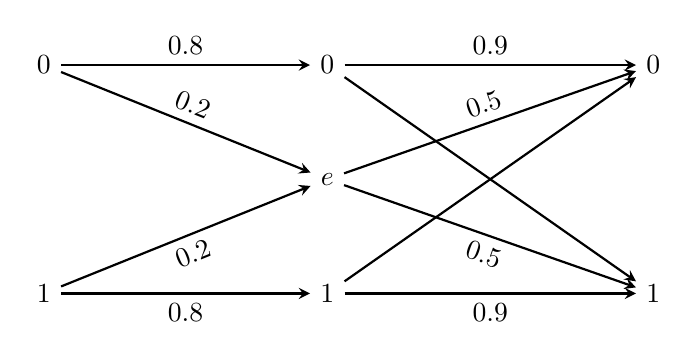
\begin{tikzpicture}[
    >=stealth,
    thick,
    x=1.8cm,
    y=1.45cm,
    every node/.style={font=\normalsize}
]

% 输入端
\node (x0) at (0,2) {$0$};
\node (x1) at (0,0) {$1$};

% 第一级信道输出端
\node (y0) at (2,2) {$0$};
\node (ye) at (2,1) {$e$};
\node (y1) at (2,0) {$1$};

% 最终输出端
\node (z0) at (4.3,2) {$0$};
\node (z1) at (4.3,0) {$1$};

% 第一级信道
\draw[->] (x0) -- node[above] {$0.8$} (y0);
\draw[->] (x0) -- node[above, sloped] {$0.2$} (ye);
\draw[->] (x1) -- node[below, sloped] {$0.2$} (ye);
\draw[->] (x1) -- node[below] {$0.8$} (y1);

% 第二级信道
\draw[->] (y0) -- node[above] {$0.9$} (z0);
\draw[->] (y0) -- node[above, sloped, pos=0.65] {} (z1);

\draw[->] (ye) -- node[above, sloped] {$0.5$} (z0);
\draw[->] (ye) -- node[below, sloped] {$0.5$} (z1);

\draw[->] (y1) -- node[below, sloped, pos=0.65] {} (z0);
\draw[->] (y1) -- node[below] {$0.9$} (z1);

\end{tikzpicture}
\end{center}

求该级联信道的等效信道矩阵，及其信道容量（保留到小数点后2位）。

\item 若上述编码后的符号0和1进行简单重复编码后再进入级联信道进行传输，即以$w_1=0000$代表0，$w_2=1111$代表1。试写出在级联信道最终输出端能使平均错误译码概率最小的译码规则，并计算平均错误译码概率。

\end{enumerate}


\newpage

\noindent
\begin{minipage}[t]{0.25\textwidth}
\renewcommand{\arraystretch}{1.5}
\begin{tabular}{|C{1.5cm}|C{2.3cm}|}
\hline
得分 & 评卷人 \\
\hline
\rule{0pt}{0.8cm}&  \\
\hline
\end{tabular}
\end{minipage}
\begin{minipage}[t]{0.72\textwidth}
\vspace{1.0cm}
\begin{center}
{\heiti 五、（6分）}
\end{center}
\end{minipage}

\vspace{1.2em}

\noindent
设某离散无记忆信源输出符号集为$U=\{-2,\,0,\,2\}$,且三个符号等概率分布。对该信源进行限失真编码，编码输出符号集为$V=\{-1,\,+1\}$.

失真函数定义为\textbf{平方误差失真}，即$d(u,v)=(u-v)^2$.


\begin{enumerate}[label=\arabic*., leftmargin=2.2em]

\item 写出该失真函数对应的失真矩阵 $D$。

\item 计算信源的\textbf{最大平均失真度} $D_{\max}$，给出能达到 $D_{\max}$ 的\textbf{试验信道}（即转移概率矩阵 $P(v|u)$）。

\item 计算信源的\textbf{最小平均失真度} $D_{\min}$，给出能达到 $D_{\min}$ 的\textbf{试验信道}（即转移概率矩阵 $P(v|u)$）。

\end{enumerate}

\newpage

\newpage

\begin{center}
{\heiti\zihao{3} 参考答案}
\end{center}

\vspace{1.5em}

\section*{一、客观题参考答案}

\begin{center}
\renewcommand{\arraystretch}{1.5}
\begin{tabularx}{\textwidth}{XXX}
1. A & 12. D & 23. A \\
2. A & 13. A & 24. A、B、C、D \\
3. C & 14. A & 25. B \\
4. A & 15. A & 26. B \\
5. B & 16. B & 27. A \\
6. B & 17. D & 28. A \\
7. A、C、D & 18. A & 29. C \\
8. B & 19. D & 30. A、B、C、D \\
9. A、B & 20. A、C & 31. B、C、D \\
10. A & 21. A & 32. B \\
11. B & 22. A & 33. B
\end{tabularx}
\end{center}

\vspace{1em}

\textbf{部分题目说明：}

第3题中，$H(Y|X)$ 表示集合 $Y$ 中除去与 $X$ 重叠部分后的区域，因此选C。

第7题中，无源数据处理最多只能保持原有信息量不变，不能增加关于原始信源的信息量，因此A、C、D正确。

第9题中，霍夫曼编码并不能使原信源符号变为近似等概率分布；当概率相同或分支标号方式不同时，得到的具体码字也不具有唯一性。霍夫曼码是即时码，并且在二进制即时码中具有最短平均码长。因此不正确的是A、B。

第11题中，由 $X\to Y\to Z$ 构成马尔可夫链，有
\[
I(XY;Z)=I(Y;Z),
\]
\[
I(X;Z)\leq I(Y;Z),
\]
以及
\[
P_{Z|X}=P_{Y|X}P_{Z|Y}.
\]

第12题中，率失真函数 $R(D)$ 是关于失真限度 $D$ 的单调不增凸函数，但不一定在整个定义域内严格递减。

第13题中，条件熵的正确计算公式应包含输入符号概率，即
\[
H(Y|X)
=
-\sum_i p(x_i)\sum_jp(y_j|x_i)\log p(y_j|x_i).
\]

第20题中，无失真信源编码的主要作用是提高通信有效性，不能直接降低信道传输错误概率。

第33题中，有噪无损信道虽然满足 $H(Y|X)>0$，但满足
\[
H(X|Y)=0,
\]
因此接收端仍可由输出唯一确定输入，实现无差错译码。


\newpage

\section*{二、循环码综合题参考答案}

已知
\[
n=7,\qquad g(x)=x^3+x+1.
\]
生成多项式的次数为
\[
n-k=3,
\]
因此该码为 $(7,4)$ 二进制循环码。

以下码字向量均按照从 $x^6$ 到 $x^0$ 的顺序排列。

\begin{enumerate}[label=\arabic*., leftmargin=2.2em]

\item \textbf{求监督多项式 $h(x)$}

在二元域 $\mathrm{GF}(2)$ 上，
\[
x^7-1=x^7+1.
\]

监督多项式满足
\[
g(x)h(x)=x^7+1.
\]

进行多项式除法可得
\[
x^7+1
=
(x^3+x+1)(x^4+x^2+x+1).
\]

因此
\[
\boxed{
h(x)=x^4+x^2+x+1
}.
\]


\item \textbf{构造标准生成矩阵 $G$ 和校验矩阵 $H$}

采用系统编码。对于信息多项式 $m(x)$，系统码字为
\[
c(x)=x^{n-k}m(x)+r(x),
\]
其中 $r(x)$ 是 $x^{n-k}m(x)$ 除以 $g(x)$ 所得的余式。

分别取信息多项式
\[
m_1(x)=x^3,\qquad
m_2(x)=x^2,\qquad
m_3(x)=x,\qquad
m_4(x)=1.
\]

计算得到
\[
x^6\bmod g(x)=x^2+1,
\]
\[
x^5\bmod g(x)=x^2+x+1,
\]
\[
x^4\bmod g(x)=x^2+x,
\]
\[
x^3\bmod g(x)=x+1.
\]

因此四个系统基码字分别为
\[
1000101,
\]
\[
0100111,
\]
\[
0010110,
\]
\[
0001011.
\]

标准生成矩阵为
\[
\boxed{
G=
\begin{bmatrix}
1&0&0&0&1&0&1\\
0&1&0&0&1&1&1\\
0&0&1&0&1&1&0\\
0&0&0&1&0&1&1
\end{bmatrix}
}.
\]

写成标准形式
\[
G=
\begin{bmatrix}
I_4&P
\end{bmatrix},
\]
其中
\[
P=
\begin{bmatrix}
1&0&1\\
1&1&1\\
1&1&0\\
0&1&1
\end{bmatrix}.
\]

在二元域上，
\[
-P^{\mathrm T}=P^{\mathrm T},
\]
所以标准校验矩阵为
\[
H=
\begin{bmatrix}
P^{\mathrm T}&I_3
\end{bmatrix}.
\]

即
\[
\boxed{
H=
\begin{bmatrix}
1&1&1&0&1&0&0\\
0&1&1&1&0&1&0\\
1&1&0&1&0&0&1
\end{bmatrix}
}.
\]

可以验证
\[
GH^{\mathrm T}=0.
\]


\item \textbf{求最小汉明距离及纠检错能力}

校验矩阵 $H$ 的每一列均为非零向量，因此不存在重量为1的非零码字。

同时，$H$ 的任意两列均不相同，因此任意两列线性无关，不存在重量为2的非零码字。

生成矩阵中存在重量为3的非零码字，例如
\[
1000101.
\]

因此
\[
\boxed{d_{\min}=3}.
\]

该码能够纠正的错误位数为
\[
t
=
\left\lfloor
\frac{d_{\min}-1}{2}
\right\rfloor
=
1.
\]

该码能够检测的错误位数为
\[
d_{\min}-1=2.
\]

所以
\[
\boxed{\text{该码能够纠正1位错误，检测至多2位错误。}}
\]


\item \textbf{对接收序列进行纠检错}

伴随式定义为
\[
S=YH^{\mathrm T}.
\]

对于
\[
Y_1=0001011,
\]
有
\[
S_1
=
Y_1H^{\mathrm T}
=
000.
\]

因此 $Y_1$ 是一个合法码字，其伴随式为零，译码器未检测到错误。

故
\[
\boxed{\widehat C_1=0001011}.
\]

由于采用系统码，前4位为信息位，因此译码结果为
\[
\boxed{\widehat M_1=0001}.
\]

对于
\[
Y_2=0101110,
\]
有
\[
S_2
=
Y_2H^{\mathrm T}
=
010.
\]

校验矩阵各列为
\[
\begin{aligned}
H_1&=101,\\
H_2&=111,\\
H_3&=110,\\
H_4&=011,\\
H_5&=100,\\
H_6&=010,\\
H_7&=001.
\end{aligned}
\]

由于
\[
S_2=H_6,
\]
在假设信道中至多发生一位错误，并采用最小重量错误图样译码时，判定第6位发生错误。

将 $Y_2$ 的第6位翻转，得到
\[
\boxed{\widehat C_2=0101100}.
\]

对应的信息序列为
\[
\boxed{\widehat M_2=0101}.
\]

\end{enumerate}


\newpage

\section*{三、马尔可夫信源综合题参考答案}

状态转移概率矩阵为
\[
P=
\begin{bmatrix}
0.8&0.2&0&0\\
0.2&0.6&0.2&0\\
0&0&0.5&0.5\\
0.8&0&0&0.2
\end{bmatrix}.
\]

\begin{enumerate}[label=\arabic*., leftmargin=2.2em]

\item \textbf{画出状态转移图}

非零状态转移概率为
\[
\begin{aligned}
&S_1\rightarrow S_1:0.8,
\qquad
S_1\rightarrow S_2:0.2,\\
&S_2\rightarrow S_1:0.2,
\qquad
S_2\rightarrow S_2:0.6,
\qquad
S_2\rightarrow S_3:0.2,\\
&S_3\rightarrow S_3:0.5,
\qquad
S_3\rightarrow S_4:0.5,\\
&S_4\rightarrow S_1:0.8,
\qquad
S_4\rightarrow S_4:0.2.
\end{aligned}
\]

状态转移图如下：

\begin{center}
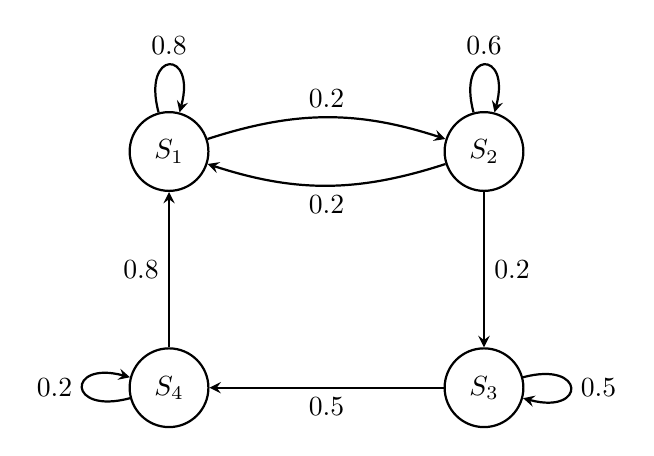
\begin{tikzpicture}[>=stealth,thick]
    \node[draw,circle,minimum size=1cm] (s1) at (0,2) {$S_1$};
    \node[draw,circle,minimum size=1cm] (s2) at (4,2) {$S_2$};
    \node[draw,circle,minimum size=1cm] (s3) at (4,-1) {$S_3$};
    \node[draw,circle,minimum size=1cm] (s4) at (0,-1) {$S_4$};

    \draw[->,loop above] (s1) to node {$0.8$} (s1);
    \draw[->,bend left=18] (s1) to node[above] {$0.2$} (s2);

    \draw[->,bend left=18] (s2) to node[below] {$0.2$} (s1);
    \draw[->,loop above] (s2) to node {$0.6$} (s2);
    \draw[->] (s2) -- node[right] {$0.2$} (s3);

    \draw[->,loop right] (s3) to node {$0.5$} (s3);
    \draw[->] (s3) -- node[below] {$0.5$} (s4);

    \draw[->,loop left] (s4) to node {$0.2$} (s4);
    \draw[->] (s4) -- node[left] {$0.8$} (s1);
\end{tikzpicture}
\end{center}


\item \textbf{求稳态分布}

设稳态分布为
\[
\boldsymbol{\pi}
=
(\pi_1,\pi_2,\pi_3,\pi_4).
\]

稳态分布满足
\[
\boldsymbol{\pi}P=\boldsymbol{\pi},
\]
以及
\[
\pi_1+\pi_2+\pi_3+\pi_4=1.
\]

由矩阵方程可得
\[
\begin{cases}
\pi_1=0.8\pi_1+0.2\pi_2+0.8\pi_4,\\
\pi_2=0.2\pi_1+0.6\pi_2,\\
\pi_3=0.2\pi_2+0.5\pi_3,\\
\pi_4=0.5\pi_3+0.2\pi_4.
\end{cases}
\]

由第二式可得
\[
0.4\pi_2=0.2\pi_1,
\]
所以
\[
\pi_2=\frac12\pi_1.
\]

由第三式可得
\[
0.5\pi_3=0.2\pi_2,
\]
所以
\[
\pi_3=\frac25\pi_2=\frac15\pi_1.
\]

由第四式可得
\[
0.8\pi_4=0.5\pi_3,
\]
所以
\[
\pi_4=\frac58\pi_3=\frac18\pi_1.
\]

利用归一化条件，
\[
\pi_1+\frac12\pi_1+\frac15\pi_1+\frac18\pi_1=1.
\]

即
\[
\frac{73}{40}\pi_1=1,
\]
所以
\[
\pi_1=\frac{40}{73}.
\]

从而
\[
\pi_2=\frac{20}{73},
\qquad
\pi_3=\frac{8}{73},
\qquad
\pi_4=\frac{5}{73}.
\]

因此稳态分布为
\[
\boxed{
\boldsymbol{\pi}
=
\left(
\frac{40}{73},
\frac{20}{73},
\frac{8}{73},
\frac{5}{73}
\right)
}.
\]

该马尔可夫链是有限、不可约且非周期的，因此为遍历链，稳态分布唯一。


\item \textbf{求信源极限熵}

一阶遍历马尔可夫信源的极限熵为
\[
H_{\infty}
=
\sum_{i=1}^{4}
\pi_i H(P_{i\cdot}),
\]
其中 $P_{i\cdot}$ 表示状态转移矩阵的第 $i$ 行。

第一行的熵为
\[
H(P_{1\cdot})
=
-0.8\log_2 0.8-0.2\log_2 0.2
=
H_2(0.2).
\]

第四行的非零概率同样为 $0.8$ 和 $0.2$，因此
\[
H(P_{4\cdot})=H_2(0.2).
\]

第二行的熵为
\[
H(P_{2\cdot})
=
-0.2\log_2 0.2
-0.6\log_2 0.6
-0.2\log_2 0.2.
\]

第三行的熵为
\[
H(P_{3\cdot})
=
-2\times0.5\log_2 0.5
=
1.
\]

数值为
\[
H_2(0.2)\approx0.721928,
\]
\[
H(0.2,0.6,0.2)\approx1.370951.
\]

因此
\[
\begin{aligned}
H_{\infty}
&=
\frac{40}{73}H_2(0.2)
+
\frac{20}{73}H(0.2,0.6,0.2)\\
&\quad+
\frac{8}{73}\times1
+
\frac{5}{73}H_2(0.2)\\
&\approx0.930216.
\end{aligned}
\]

所以
\[
\boxed{
H_{\infty}
\approx
0.9302\ \text{bit/符号}
}.
\]


\item \textbf{求 $\displaystyle\lim_{n\to\infty}P^n$}

由于该马尔可夫链为有限遍历链，当 $n\to\infty$ 时，矩阵 $P^n$ 的每一行都趋于稳态分布。

因此
\[
\boxed{
\lim_{n\to\infty}P^n
=
\begin{bmatrix}
\dfrac{40}{73}&\dfrac{20}{73}&\dfrac{8}{73}&\dfrac{5}{73}\\[0.5em]
\dfrac{40}{73}&\dfrac{20}{73}&\dfrac{8}{73}&\dfrac{5}{73}\\[0.5em]
\dfrac{40}{73}&\dfrac{20}{73}&\dfrac{8}{73}&\dfrac{5}{73}\\[0.5em]
\dfrac{40}{73}&\dfrac{20}{73}&\dfrac{8}{73}&\dfrac{5}{73}
\end{bmatrix}
}.
\]

\end{enumerate}


\newpage

\section*{四、信源编码与级联信道参考答案}

\begin{enumerate}[label=\arabic*., leftmargin=2.2em]

\item \textbf{设计编码方案并分析编码效率}

各符号概率为
\[
\begin{array}{c|ccccc}
\text{类别}&A&B&C&D&E\\
\hline
p&0.30&0.25&0.20&0.15&0.10
\end{array}.
\]

使用二进制霍夫曼编码。

首先合并概率最小的两个符号：
\[
0.10+0.15=0.25.
\]

此时概率为
\[
0.20,\quad0.25,\quad0.25,\quad0.30.
\]

再合并
\[
0.20+0.25=0.45.
\]

剩余概率为
\[
0.25,\quad0.30,\quad0.45.
\]

再合并
\[
0.25+0.30=0.55.
\]

最后合并
\[
0.45+0.55=1.
\]

一种可行的霍夫曼编码为
\[
\begin{array}{c|ccccc}
\text{类别}&A&B&C&D&E\\
\hline
\text{码字}&10&01&00&110&111\\
\text{码长}&2&2&2&3&3
\end{array}.
\]

该码满足前缀条件，因此是即时码。

平均码长为
\[
\begin{aligned}
\overline L
&=
0.30\times2
+
0.25\times2
+
0.20\times2\\
&\quad+
0.15\times3
+
0.10\times3\\
&=2.25.
\end{aligned}
\]

因此
\[
\boxed{
\overline L=2.25\ \text{bit/符号}
}.
\]

信源熵为
\[
H(S)
=
-\sum_i p_i\log_2p_i.
\]

即
\[
\begin{aligned}
H(S)
={}&
-0.30\log_2 0.30
-0.25\log_2 0.25\\
&-0.20\log_2 0.20
-0.15\log_2 0.15
-0.10\log_2 0.10\\
\approx{}&2.2282\ \text{bit/符号}.
\end{aligned}
\]

编码效率为
\[
\eta
=
\frac{H(S)}{\overline L}
=
\frac{2.2282}{2.25}
\approx0.9903.
\]

所以
\[
\boxed{\eta\approx99.03\%}.
\]


\item \textbf{求等效信道矩阵及信道容量}

令第一级信道的输入为 $X$，输出为 $Y$，第二级信道输出为 $Z$。

第一级信道的输入字母顺序取为
\[
X=(0,1),
\]
输出字母顺序取为
\[
Y=(0,e,1).
\]

则第一级信道矩阵为
\[
P_{Y|X}
=
\begin{bmatrix}
0.8&0.2&0\\
0&0.2&0.8
\end{bmatrix}.
\]

第二级信道中，图中两条未标注的交叉支路概率均为
\[
1-0.9=0.1.
\]

因此
\[
P_{Z|Y}
=
\begin{bmatrix}
0.9&0.1\\
0.5&0.5\\
0.1&0.9
\end{bmatrix}.
\]

级联信道的等效转移概率矩阵为
\[
P_{Z|X}
=
P_{Y|X}P_{Z|Y}.
\]

于是
\[
\begin{aligned}
P_{Z|X}
&=
\begin{bmatrix}
0.8&0.2&0\\
0&0.2&0.8
\end{bmatrix}
\begin{bmatrix}
0.9&0.1\\
0.5&0.5\\
0.1&0.9
\end{bmatrix}\\
&=
\begin{bmatrix}
0.82&0.18\\
0.18&0.82
\end{bmatrix}.
\end{aligned}
\]

所以等效信道为交叉概率
\[
p=0.18
\]
的二进制对称信道。

等效信道矩阵为
\[
\boxed{
P_{Z|X}
=
\begin{bmatrix}
0.82&0.18\\
0.18&0.82
\end{bmatrix}
}.
\]

二进制对称信道的容量为
\[
C=1-H_2(p).
\]

因此
\[
\begin{aligned}
C
&=
1-H_2(0.18)\\
&=
1+0.18\log_2 0.18
+0.82\log_2 0.82\\
&\approx0.3199.
\end{aligned}
\]

保留到小数点后两位，
\[
\boxed{
C\approx0.32\ \text{bit/次信道使用}
}.
\]


\item \textbf{求最小平均错误概率译码规则及错误概率}

采用四次重复码
\[
w_1=0000,
\qquad
w_2=1111.
\]

等效信道为交叉概率
\[
p=0.18
\]
的二进制对称信道。

题目未给出0和1的先验概率，因此按照等概率输入处理，即
\[
P(w_1)=P(w_2)=\frac12.
\]

对于接收序列
\[
Z=(z_1,z_2,z_3,z_4),
\]
令其汉明重量为
\[
w_H(Z)=\sum_{i=1}^{4}z_i.
\]

因为
\[
p<\frac12,
\]
最小平均错误概率译码等价于最大似然译码，也等价于最小汉明距离译码。

译码规则为
\[
\boxed{
\begin{cases}
w_H(Z)<2,&\widehat w=w_1=0000,\\
w_H(Z)>2,&\widehat w=w_2=1111,\\
w_H(Z)=2,&\text{随机判决，或固定判给任一码字。}
\end{cases}
}
\]

具体而言：
\[
0000,\ 0001,\ 0010,\ 0100,\ 1000
\]
译为 $w_1$；

\[
1111,\ 1110,\ 1101,\ 1011,\ 0111
\]
译为 $w_2$；

其余6个重量为2的序列处于判决边界。

设4位中发生错误的位数为 $K$，则
\[
K\sim\operatorname{\textit{B}}(4,0.18).
\]

当错误位数大于2时一定译码错误；当错误位数等于2时，随机判决有一半概率译码错误。因此
\[
P_e
=
P(K\geq3)
+
\frac12P(K=2).
\]

于是
\[
\begin{aligned}
P_e
={}&
\mathrm{C}_4^3(0.18)^3(0.82)
+
\mathrm{C}_4^4(0.18)^4\\
&+
\frac12\mathrm{C}_4^2(0.18)^2(0.82)^2.
\end{aligned}
\]

计算得
\[
P_e=0.085536.
\]

因此
\[
\boxed{
P_e\approx0.0855=8.55\%
}.
\]

\end{enumerate}


\newpage

\section*{五、限失真编码参考答案}

信源符号集为
\[
U=\{-2,0,2\},
\]
各符号等概率，即
\[
p(-2)=p(0)=p(2)=\frac13.
\]

再现符号集为
\[
V=\{-1,+1\}.
\]

失真函数为
\[
d(u,v)=(u-v)^2.
\]

以下失真矩阵的行按照
\[
u=-2,0,2
\]
排列，列按照
\[
v=-1,+1
\]
排列。

\begin{enumerate}[label=\arabic*., leftmargin=2.2em]

\item \textbf{写出失真矩阵}

各元素为
\[
d(-2,-1)=1,
\qquad
d(-2,+1)=9,
\]
\[
d(0,-1)=1,
\qquad
d(0,+1)=1,
\]
\[
d(2,-1)=9,
\qquad
d(2,+1)=1.
\]

因此失真矩阵为
\[
\boxed{
D=
\begin{bmatrix}
1&9\\
1&1\\
9&1
\end{bmatrix}
}.
\]


\item \textbf{求最大平均失真度 $D_{\max}$}

在率失真理论中，
\[
D_{\max}
=
\min_{v\in V}
\sum_{u\in U}p(u)d(u,v).
\]

若始终输出
\[
v=-1,
\]
则平均失真为
\[
\begin{aligned}
\overline D_{-1}
&=
\frac13
\left[
d(-2,-1)+d(0,-1)+d(2,-1)
\right]\\
&=
\frac13(1+1+9)\\
&=
\frac{11}{3}.
\end{aligned}
\]

若始终输出
\[
v=+1,
\]
则平均失真为
\[
\begin{aligned}
\overline D_{+1}
&=
\frac13
\left[
d(-2,+1)+d(0,+1)+d(2,+1)
\right]\\
&=
\frac13(9+1+1)\\
&=
\frac{11}{3}.
\end{aligned}
\]

因此
\[
\boxed{
D_{\max}=\frac{11}{3}
}.
\]

一种能够达到 $D_{\max}$ 的试验信道为始终输出 $v=-1$，即
\[
\boxed{
P(v|u)
=
\begin{bmatrix}
1&0\\
1&0\\
1&0
\end{bmatrix}
}.
\]

其中每一行依次对应
\[
u=-2,0,2,
\]
两列依次对应
\[
v=-1,+1.
\]

同理，始终输出 $v=+1$ 也可以达到 $D_{\max}$：
\[
P(v|u)
=
\begin{bmatrix}
0&1\\
0&1\\
0&1
\end{bmatrix}.
\]

更一般地，只要输出与输入无关，即
\[
P(v|u)
=
\begin{bmatrix}
q&1-q\\
q&1-q\\
q&1-q
\end{bmatrix},
\qquad
0\leq q\leq1,
\]
均有
\[
\overline D=\frac{11}{3}.
\]


\item \textbf{求最小平均失真度 $D_{\min}$}

对每一个信源符号，选择使失真最小的再现符号。

当
\[
u=-2
\]
时，应选择
\[
v=-1,
\]
最小失真为
\[
1.
\]

当
\[
u=0
\]
时，选择 $v=-1$ 或 $v=+1$ 的失真均为
\[
1.
\]

当
\[
u=2
\]
时，应选择
\[
v=+1,
\]
最小失真为
\[
1.
\]

因此
\[
\begin{aligned}
D_{\min}
&=
\sum_u p(u)\min_v d(u,v)\\
&=
\frac13(1+1+1)\\
&=1.
\end{aligned}
\]

所以
\[
\boxed{D_{\min}=1}.
\]

一种能够达到 $D_{\min}$ 的试验信道为
\[
-2\mapsto-1,
\qquad
0\mapsto-1,
\qquad
2\mapsto+1.
\]

对应的转移概率矩阵为
\[
\boxed{
P(v|u)
=
\begin{bmatrix}
1&0\\
1&0\\
0&1
\end{bmatrix}
}.
\]

由于 $u=0$ 到 $v=-1$ 和 $v=+1$ 的失真均为1，因此更一般的最优试验信道可以写为
\[
\boxed{
P(v|u)
=
\begin{bmatrix}
1&0\\
\alpha&1-\alpha\\
0&1
\end{bmatrix},
\qquad
0\leq\alpha\leq1
}.
\]

\end{enumerate}





\end{document}
